\documentclass[12pt,a4paper]{report}

%\usepackage[a4paper]{geometry}
%\usepackage{showframe}
\usepackage[english,russian]{babel}
\usepackage[T1,T2A]{fontenc}
\usepackage[utf8]{inputenc}
\usepackage{amsmath}
\usepackage{amssymb}
\usepackage{mathtools}
\usepackage[center]{caption}
\usepackage[caption2]{ccaption}
\usepackage{indentfirst}
\usepackage{setspace}
\usepackage{etoolbox}
\usepackage{todonotes}
\usepackage{url}

\renewcommand{\contentsname}{Содержание}
\renewcommand{\bibname}{Список литературы}
\renewcommand{\figurename}{Рис.}
\renewcommand{\tablename}{Таблица}
\renewcommand{\abstractname}{Аннотация}
\renewcommand{\partname}{Часть}

\renewcommand{\bottomfraction}{0.5}
\renewcommand{\floatpagefraction}{0.4}
\renewcommand{\textfloatsep}{0.5cm}
\renewcommand{\intextsep}{0.6cm}
\renewcommand{\floatsep}{0.3cm}

\hoffset -1.0cm
\textwidth  16.5cm
\textheight 24cm

% refs
\newcommand\figref[1]{(рис. \ref{#1})}
% for todos
\newcommand\note[1]{\textcolor{red}{(#1)}}
\newcommand\todonote[1]{\note{TODO: #1}}

\begin{document}

% Титульный лист
\begin{titlepage}
\par
\vspace*{-4cm}
\begin{center}
{\large

Санкт-Петербургский Государственный Политехнический Университет\\
Институт прикладной математики и механики\\
Кафедра прикладной математики\\

\vspace*{0.5cm}

\begin{flushright}
Диссертация допущена к защите\\
Зав. кафедрой\ \ \ \ \ \ \ \ \ \ \ \ \ \ \ \ \ \ \ \ \ \ \ \ \ \ \ \\
\underline{ \ \ \ \ \ \ \ \ \ \ \ \ \ \ \ \ \ \ \ \ \ \ \ \ \ \ \ \ \ \ \ \ \ \ \ \ \ \ \ \ \ \ \ } \\
"\underline{ \ \ \ }"\underline{ \ \ \ \ \ \ \ \ \ \ \ \ \ \ \ \ \ \ \ \ \ \ \ \ \ \ \ \ \ \ \ \ \ \ \ \ \ }
\end{flushright}

\vspace*{2.0cm}

{\Large
  \textbf{
    ДИССЕРТАЦИЯ\\
    на соискание степени МАГИСТРА\\
  }
}
\vspace*{1cm}
\textbf{
  Тема: \emph{метод ранжирования разнородных результатов поиска}\\
}

}

\vspace*{1.5cm}

\begin{flushleft}
Направление: 01.04.02 - Прикладная математика и информатика\\
Магистерская программа: системное программирование\\
\end{flushleft}

\vspace*{1cm}

Выполнил студент гр. 63601/2 \ \ \ \ \ \ \ \ \ \ \ \ \ \ \ \ \ \ \ \ \ \ \ \ \ \ \ \ \ \ \ \ \ \ \ \ \ \underline{ \ \ \ \ \ \ \ \ \ \ \ \ \ \ \ \ \ \ \ \ \ \ \ } Толмачев А.С.\\
\vspace*{0.3cm}
Руководитель, к.ф.-м.н., доц. \ \ \ \ \ \ \ \ \ \ \ \ \ \ \ \ \ \ \ \ \ \ \ \ \ \ \ \ \ \ \ \ \ \ \ \ \ \ \underline{ \ \ \ \ \ \ \ \ \ \ \ \ \ \ \ \ \ \ \ \ \ \ \ } Иванков А.А.
\vspace*{0.5cm}

\vspace*{0.3cm}

\begin{flushleft}
Консультанты:\\
\vspace*{0.3cm}
по вопросам информационного поиска, к.ф.-м.н. \ \ \ \ \ \ \underline{ \ \ \ \ \ \ \ \ \ \ \ \ \ \ \ \ \ \ \ \ \ \ \ } Кураленок И.Е.\\
\vspace*{0.3cm}
по вопросам охраны труда, к.т.н., доц. \ \ \ \ \ \ \ \ \ \ \ \ \ \ \ \ \ \ \ \ \underline{ \ \ \ \ \ \ \ \ \ \ \ \ \ \ \ \ \ \ \ \ \ \ \ } Монашков В.В.
\end{flushleft}

\end{center}
\vfill
\begin{center}
{\large Санкт-Петербург \\ 2015}
\end {center}
\end{titlepage}

\hoffset 0.46cm
\marginparsep 0pt
\oddsidemargin 0pt
\textwidth 16.5cm
\topmargin -1.5cm
\textheight 9.5in
\footskip 40pt
\parindent 1cm

% 1.5 line spacing
%\renewcommand{\baselinestretch}{1.5}
\setstretch{1.5}
% Use 1.0 spacing for chapter headings
\makeatletter
\patchcmd{\@makechapterhead}{\huge}{\setstretch{1.0}\huge}{}{}
\apptocmd{\@makechapterhead}{}{}{}
\makeatother

\pagenumbering{arabic}
\setcounter{tocdepth}{4}
\normalsize

%=================================================================
\renewcommand{\contentsname}{Содержание}
\tableofcontents

%=================================================================
\chapter*{Введение}
\addcontentsline{toc}{chapter}{Введение}

% План:
% Мотивация
% - о важности информационного поиска и поисковых систем
% - о важности задачи ранжирования
% - о развитии поисковых систем (тренд -- внедрение результатов вертикальных поисков) + специализированные результаты для сценариев
% - о задаче ранжирования разнородных результатов

% Важность информации в современном мире -> С развитием информационных технологий стало доступно огромное количество информации, Интернет -> надо искать в этом огромном море информации -> поисковые системы имеют очень большую важность для людей сегодня, стали неотъемлемой частью нашей жизни

C развитием информационных систем и ростом их популярности растет и количество информации, производимой с их помощью. Так, по данным аналитической компании IDC (International Data Corporation) общий объем цифровой информации в мире составил на 2013 год примерно 4.4 зеттабайт\footnote{1 зеттабайт (ЗБ) = 1 триллион гигабайт}, он увеличивается каждый год примерно на 40\% и к 2020 году составит приблизительно 44 зеттабайт \cite{IDC-Analytics}. Существенная доля этой информации -- информация, размещенная во всемирной сети Интернет. Она большей частью неструктурирована и очень разнообразна. Несомненно, без помощи поисковых систем ориентироваться в этом огромном информационном пространстве не представляется возможным. Поэтому системы веб-поиска на сегодняшний день играют очень важную роль в нашей жизни.

C момента своего возникновения веб-поисковые системы активно развиваются. Одно из современных направлений их развития касается смешивания в результатах поиска разнотипной информации. Первые системы поиска в интернете в ответ на запрос выдавали список ссылок на веб-страницы \figref{early-search-engines} \cite{SearchHistory}.
\begin{figure}[]
  \centering
  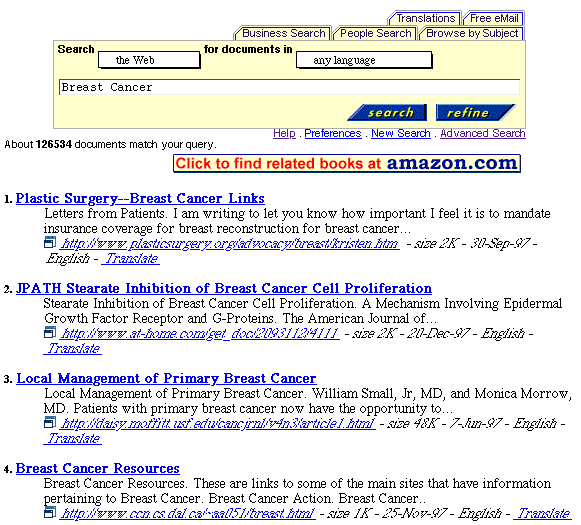
\includegraphics[height=0.3\textheight]{pics/AltavistaResults.png}
  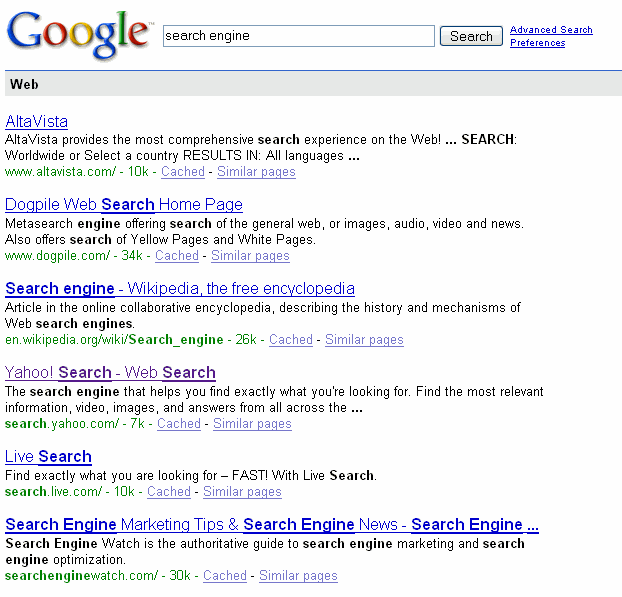
\includegraphics[height=0.3\textheight]{pics/Google-EarlyResults.png}
  \caption{Страницы результатов поиска системы AltaVista и одной из первых версий системы Google.}
  \label{early-search-engines}
\end{figure}
Такой вид результатов поиска для того времени был естественным, поскольку представляемая в них информация была однотипной.
% достаточно однородной?
% \note{почему?}
% поскольку информация, содержащаяся в интернете на заре его истории, не отличалась большим разнообразием. 
%Ограничение результатов поиска одним типом -- веб-страницами -- было естественным, поскольку в то время интернет по сути представлял собой набор текстовых страниц, ссылающихся друг на друга при помощи гиперссылок \note{не по этому?}. 
Но по мере того, как развивались интернет-технологии и увеличивалось число интернет-пользователей, информация, размещаемая в сети, становилось все более разнообразной. На сегодняшний день это разнообразие огромно: в интернете можно найти музыку, фильмы, новости, тексты книг, научные статьи, программные приложения, кулинарные рецепты, технические характеристики товаров и отзывы о них и т. д. -- все это различные типы информации. В связи с этим получили развитие системы, предназначенные для агрегации и поиска информации определенного типа. К таковым относятся, например, системы поиска изображений, видео-записей, новостей, товаров, музыки. 
Ясно, что такая специализированная система может быть более удобной и полезной для решения поисковой задачи из соответствующей области, чем система общего назначения. 
%которая на любой запрос выдает список интернет-страниц. 
Действительно, если пользователь, к примеру, ищет фотографии Дворцовой площади, то, очевидно, ему будет гораздо удобнее, если в качестве результатов поиска он будет видеть именно фотографии, а не ссылки на веб-страницы -- ему не нужно будет переходить по этим ссылкам и самостоятельно исследовать страницы в поисках фотографий.
Но выбирать каждый раз, к какой из многочисленных специализированных систем обратиться, неудобно. К тому же пользователь может не знать о существовании той или иной специализированной системы, а для каких-то поисковых задач такой системы может и не быть. Поэтому возникает естественное желание, чтобы система веб-поиска сама ``понимала'' запрос пользователя, и выдавала в ответ информацию нужного типа. Однако ограничивать ответ на запрос каким-то одним типом информации также неоправданно -- для решения своей поисковой задачи пользователю может быть полезна информация сразу нескольких типов. Так, например, при поиске информации о музыкальном исполнителе может быть полезна и его биография, и фотографии с ним, и аудио-записи исполняемой им музыки, и видео-сюжеты о нем. Или же поисковый запрос может быть многозначным -- например, по запросу ``политика'' пользователя может интересовать как информация, касающаяся самого термина, так и политические новости. 
Стандартным на сегодняшний день решением является смешивание результатов поиска от разных специализированных систем и представление их вместе с традиционными результатами веб-поиска -- списком ссылок на интернет-страницы. Такое смешивание мы можем наблюдать, пользуясь современными поисковыми системами. Например, в результатах поиска систем Яндекс и Google можно увидеть разнообразные специализированные результаты: на поисковый запрос о картинах -- результаты поиска по изображениям, на запрос об адресе в городе --  интерактивную карту с отмеченным адресом, на запрос о новостях -- результаты поиска по новостям, а на запрос о кафе -- специализированный ответ с найденными заведениями и информацией о них \figref{vertical-results}. 
% Такие специализированные результаты позволяют пользователю получить интересующую его информацию сразу же на странице с результатами поиска или перейти в специализированную поисковую систему и продолжить поиск информации с ее помощью.
Таким образом, результаты поиска могут быть \emph{разнородными}, поскольку могут содержать информацию разных типов.

\begin{figure}[b!]
  \centering
  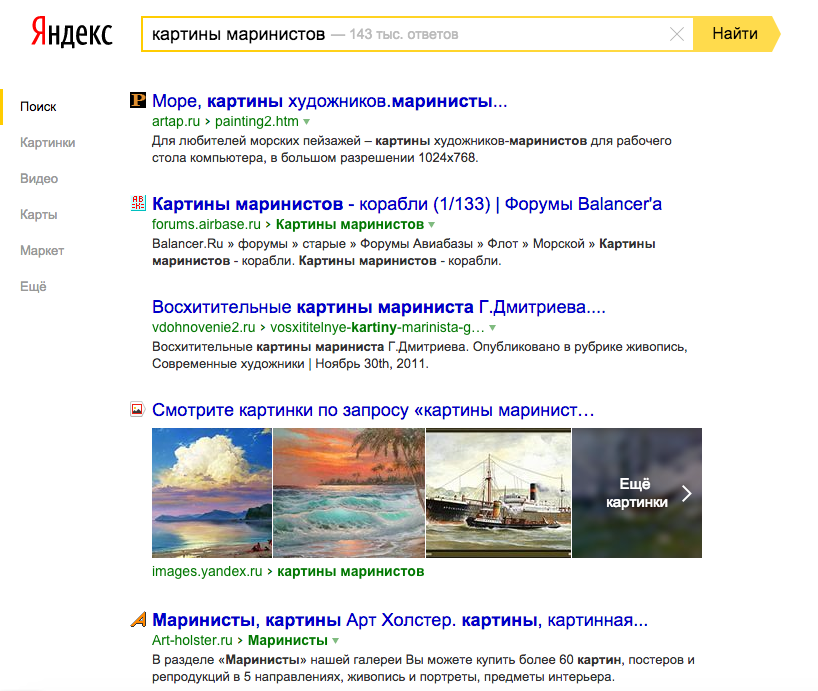
\includegraphics[height=0.27\textheight]{pics/VerticalResults-Images-Yandex.png}
  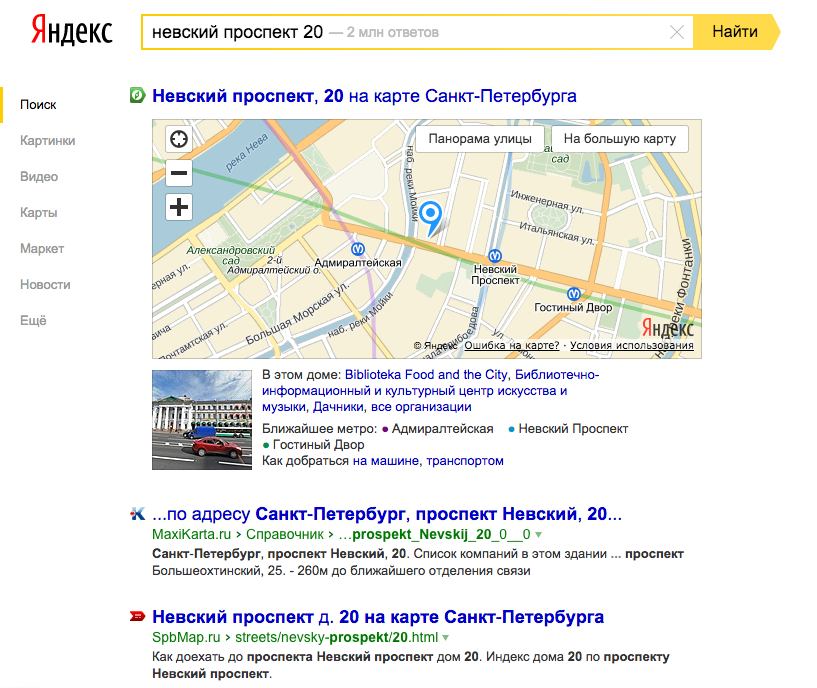
\includegraphics[height=0.27\textheight]{pics/VerticalResults-Maps-Yandex.png}
  \vfill\vfill
  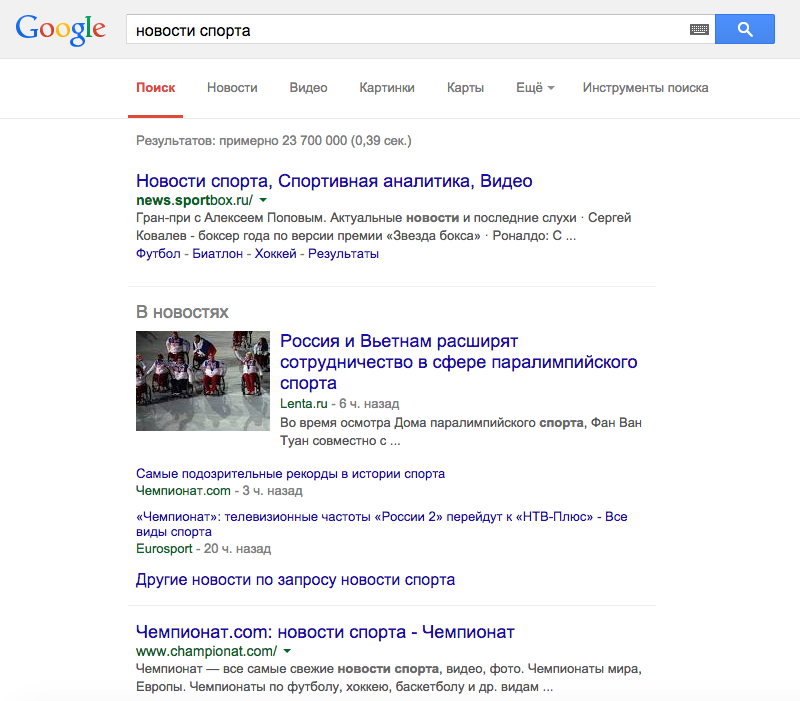
\includegraphics[height=0.27\textheight]{pics/VerticalResults-News-Google.png}
  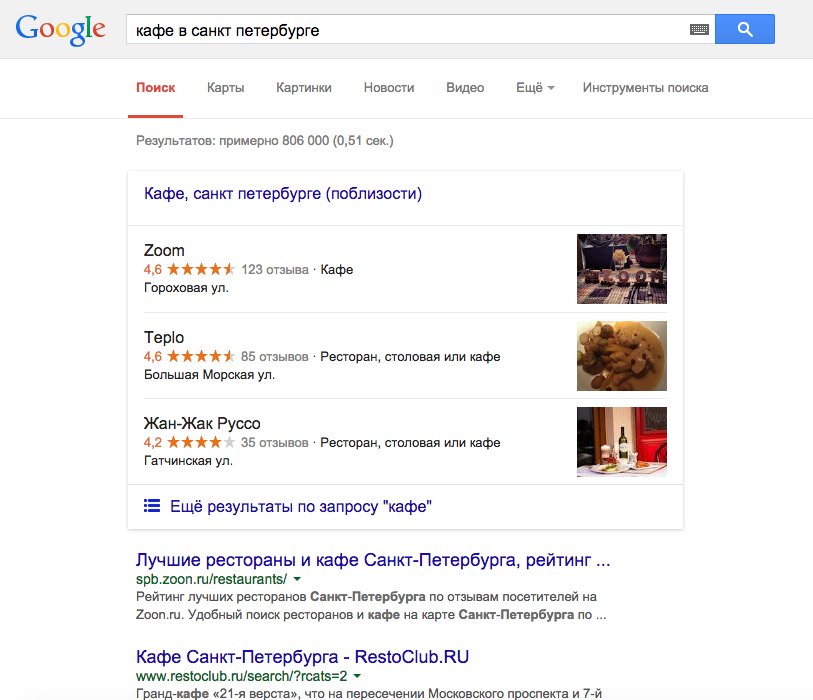
\includegraphics[height=0.27\textheight]{pics/VerticalResults-Places-Google.png}
  \caption{Специализированные ответы в результатах поиска систем Яндекс и Google.}
  \label{vertical-results}
\end{figure}

Процесс обработки поискового запроса можно условно разделить на два этапа: поиск информации, соответствующей запросу, и представление найденной информации.
На первом этапе из всего множества объектов, известных системе, выбираются те, которые по тем или иным критериям соответствуют заданному запросу. На втором этапе множество найденных объектов представляется некоторым образом и выдается пользователю. 
% Результаты поиска, представленные определенным образом, называются \emph{поисковой выдачей}. 
Задача \emph{ранжирования} относится ко второму из этих этапов. Ранжирование -- это упорядочение результатов поиска в соответствии с некоторым принципом \cite{Ashmanov, LiuLR}. От того, как упорядочены результаты, во многом зависит то, насколько успешно пользователь сможет решить свою поисковую задачу. 
%Например, если результаты представляются в виде списка, то было бы разумно стараться располагать те из них, которые могут быть наиболее полезны пользователю в контексте заданного им запроса, в начале списка, а менее полезные -- в конце.  
Так, например, если пользователь задал запрос ``скалолазание википедия'', то, вероятно, он ищет статью о скалолазании из интернет-энциклопедии Википедия. Если среди найденных результатов эта статья присутствует, то разумно расположить ее первой в списке результатов поиска, чтобы пользователь смог сразу ею воспользоваться. В противном случае ему будет сложнее найти этот результат среди остальных, а если расположить его за пределами первых десяти результатов, то он и вовсе может решить, что эта статья не была найдена. Каждый из специализированных ответов, встраиваемых в результаты поиска, также может быть более или менее полезен пользователю в сравнении с другими результатами при решении своей поисковой задачи. 
%Поэтому их также требуется ранжировать.
Кроме этого, какие-то из специализированных ответов могут быть в принципе не уместны для заданного поискового запроса. Таким образом, возникает задача выбора специализированных результатов для показа по запросу и ранжирования их в поисковой выдаче. 
%При встраивании в результаты поиска специализированных ответов их также требуется ранжировать -- каждый из специализированных ответов может быть более или менее полезен пользователю в сравнении с другими результатами.

Задача ранжирования, возникающая при смешивании специализированных ответов с традиционными результатами веб-поиска, существенно отличается от классической задачи ранжирования \cite{LiuLR}. 
Во-первых, классическая задача формулируется для однотипных объектов, в то время как в рассматриваемой задаче ранжируемые результаты разнородны.
Во-вторых, специализированные ответы встраиваются только на первую страницу результатов поиска, поэтому количество ранжируемых объектов при этом невелико. Эти отличия, в особенности первое их них, не позволяют применить для решения рассматриваемой задачи существующие методы решения классической задачи. Соответственно, требуется либо их обобщение, либо разработка принципиально новых подходов.

\begin{figure}[t!]
  \centering
  
\includegraphics[width=0.9\textwidth]{pics/EntitySearch-Google.png}
  \caption{Поисковая выдача системы Google со специализированным результатом в отдельной колонке.}
  \label{two-coloumn-serp}
\end{figure}

% Разные модели поисковой выдачи, особенности, связанные с этим
Также следует отметить, что список, -- не единственный способ представления результатов поиска. Модели поисковой выдачи могут быть различными. Например, поисковая выдача системы Google для настольных компьютеров имеет две колонки, в левой из которых располагается список результатов, а в правой могут располагаться специализированные ответы \figref{two-coloumn-serp}. А выдача мобильного приложения поисковой системы Яндекс состоит из страниц, каждая из которых может содержать список результатов или специализированные ответы. Набор этих страниц и их порядок зависит от запроса \figref{yandex-mobile-app-serp}. В таких случаях задача ранжирования усложняется и превращается в задачу расположения результатов поиска в соответствии с заданной моделью поисковой выдачи. Это также требует обобщения существующих методов ранжирования.

\begin{figure}[b!]
  \centering
  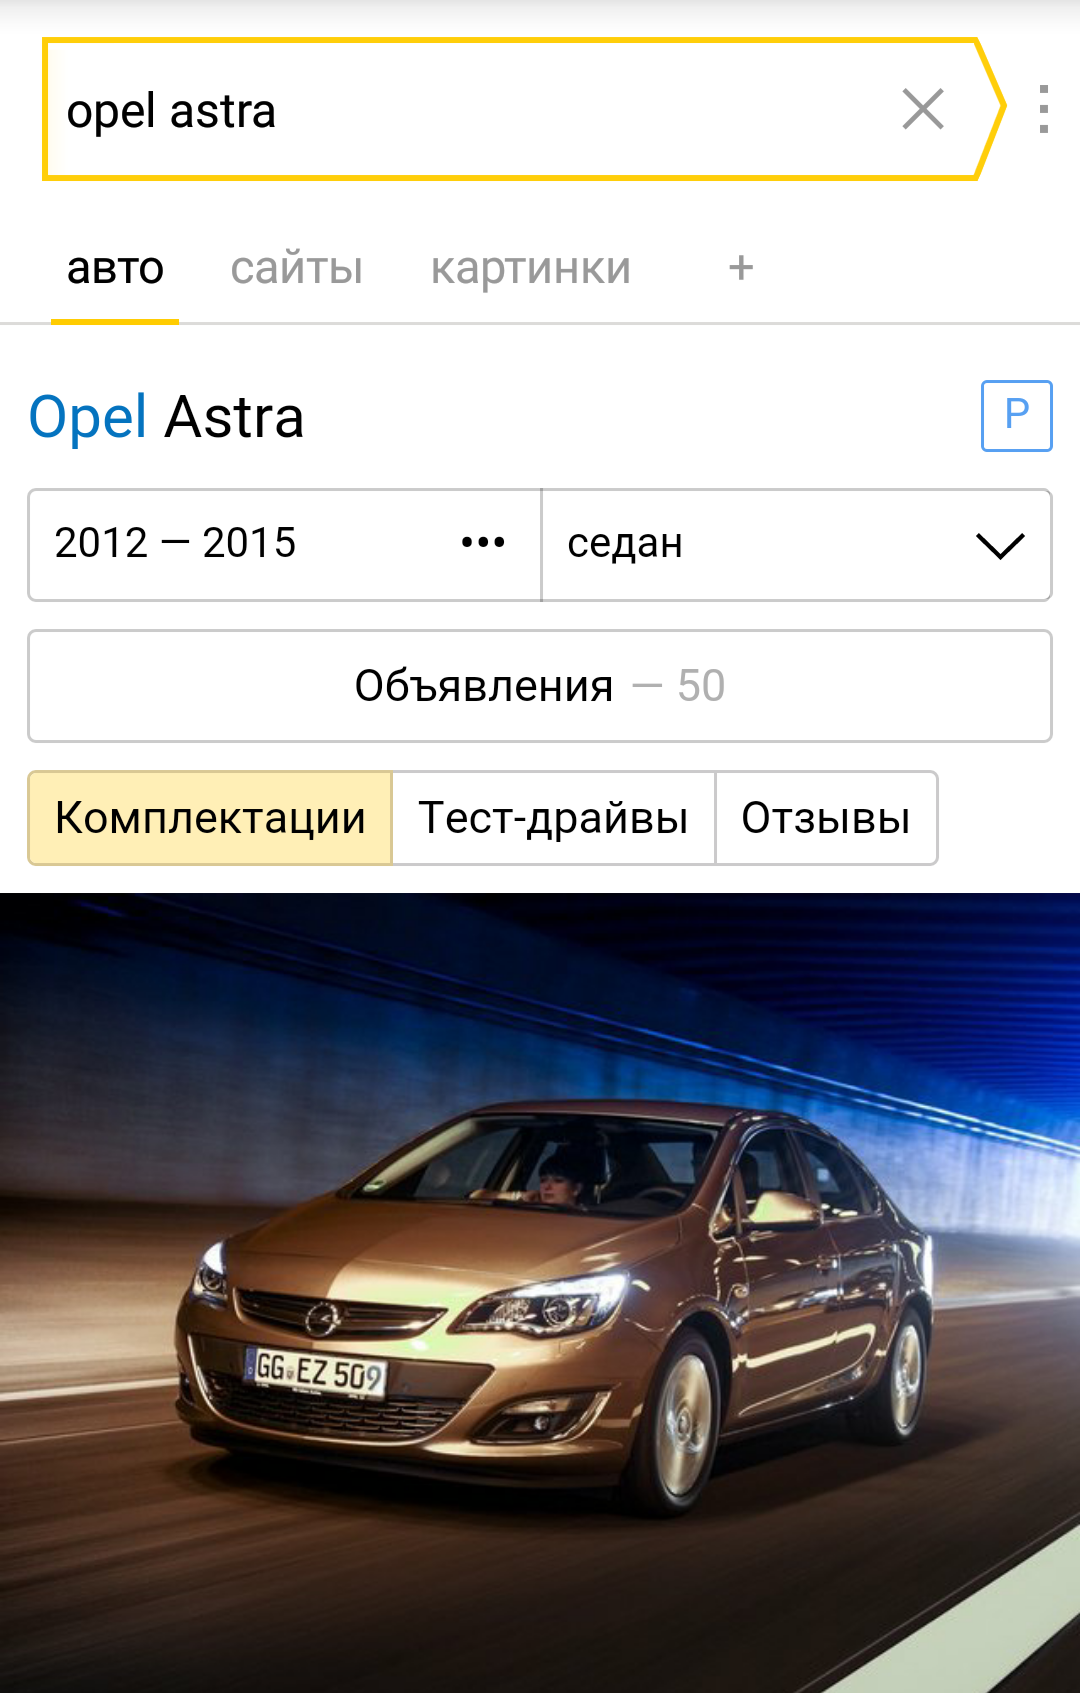
\includegraphics[width=0.3\textwidth]{pics/MultiPageSerp-Yandex-1.png}
  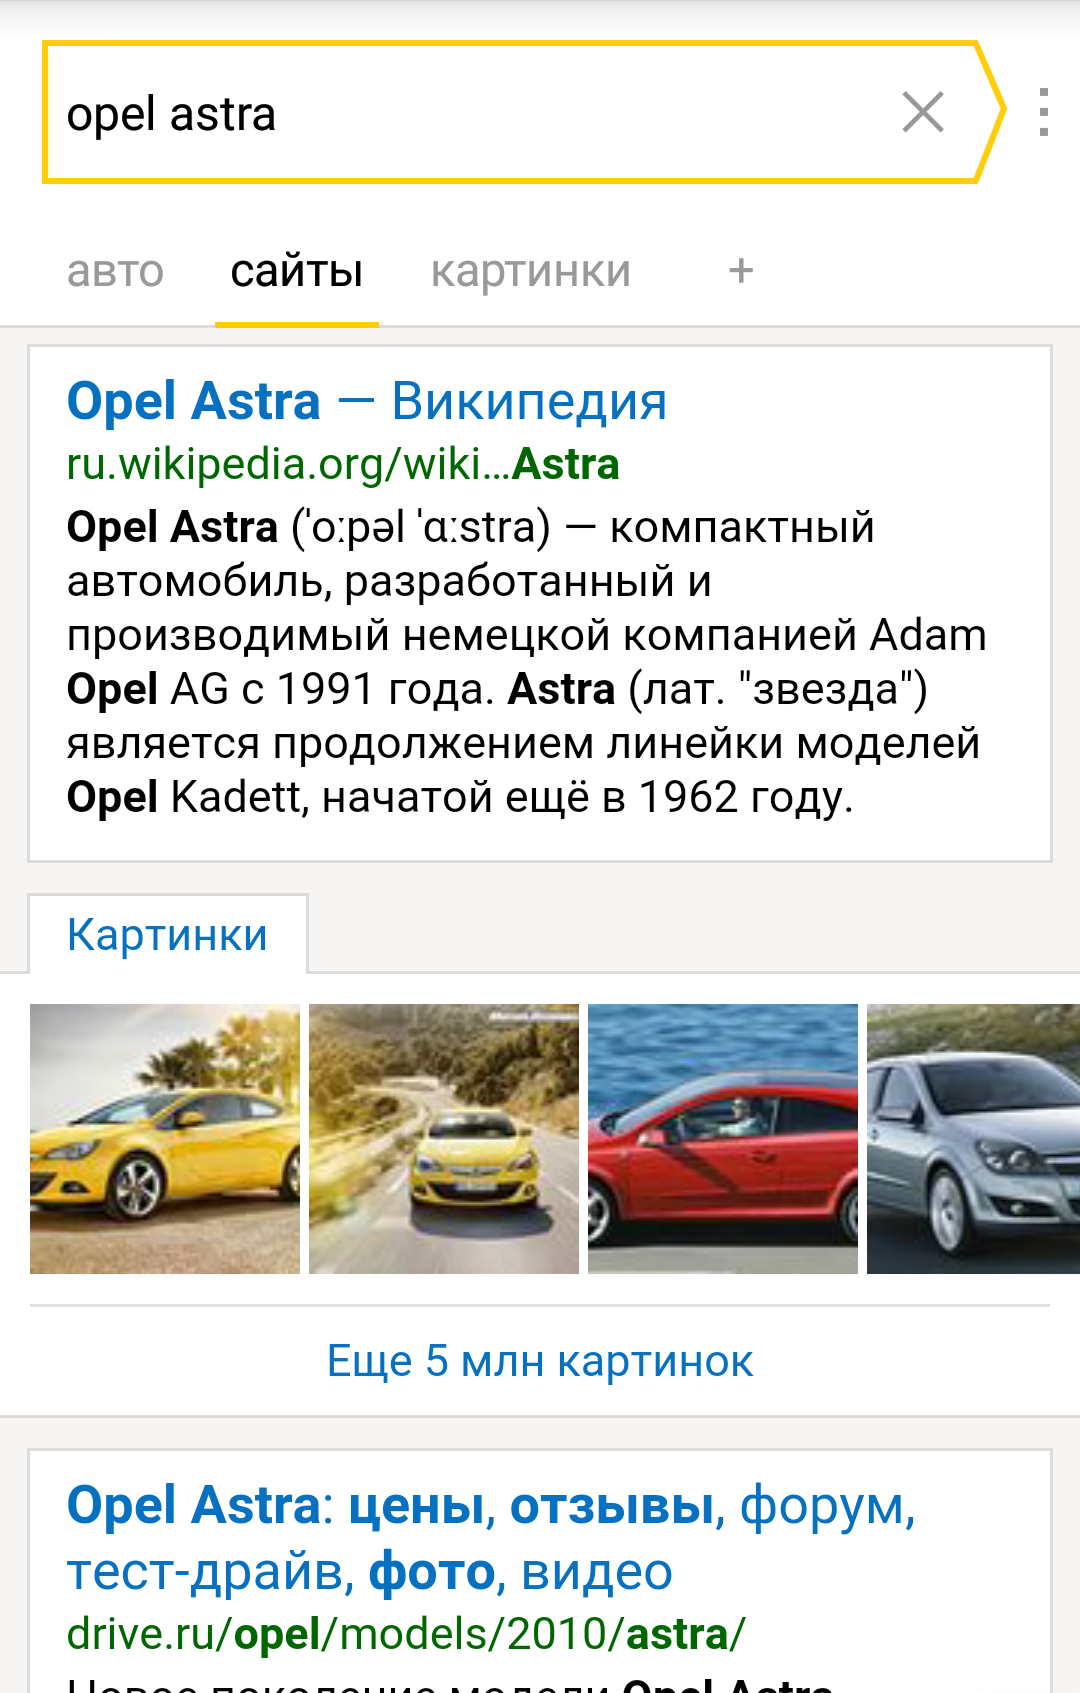
\includegraphics[width=0.3\textwidth]{pics/MultiPageSerp-Yandex-2.png}
  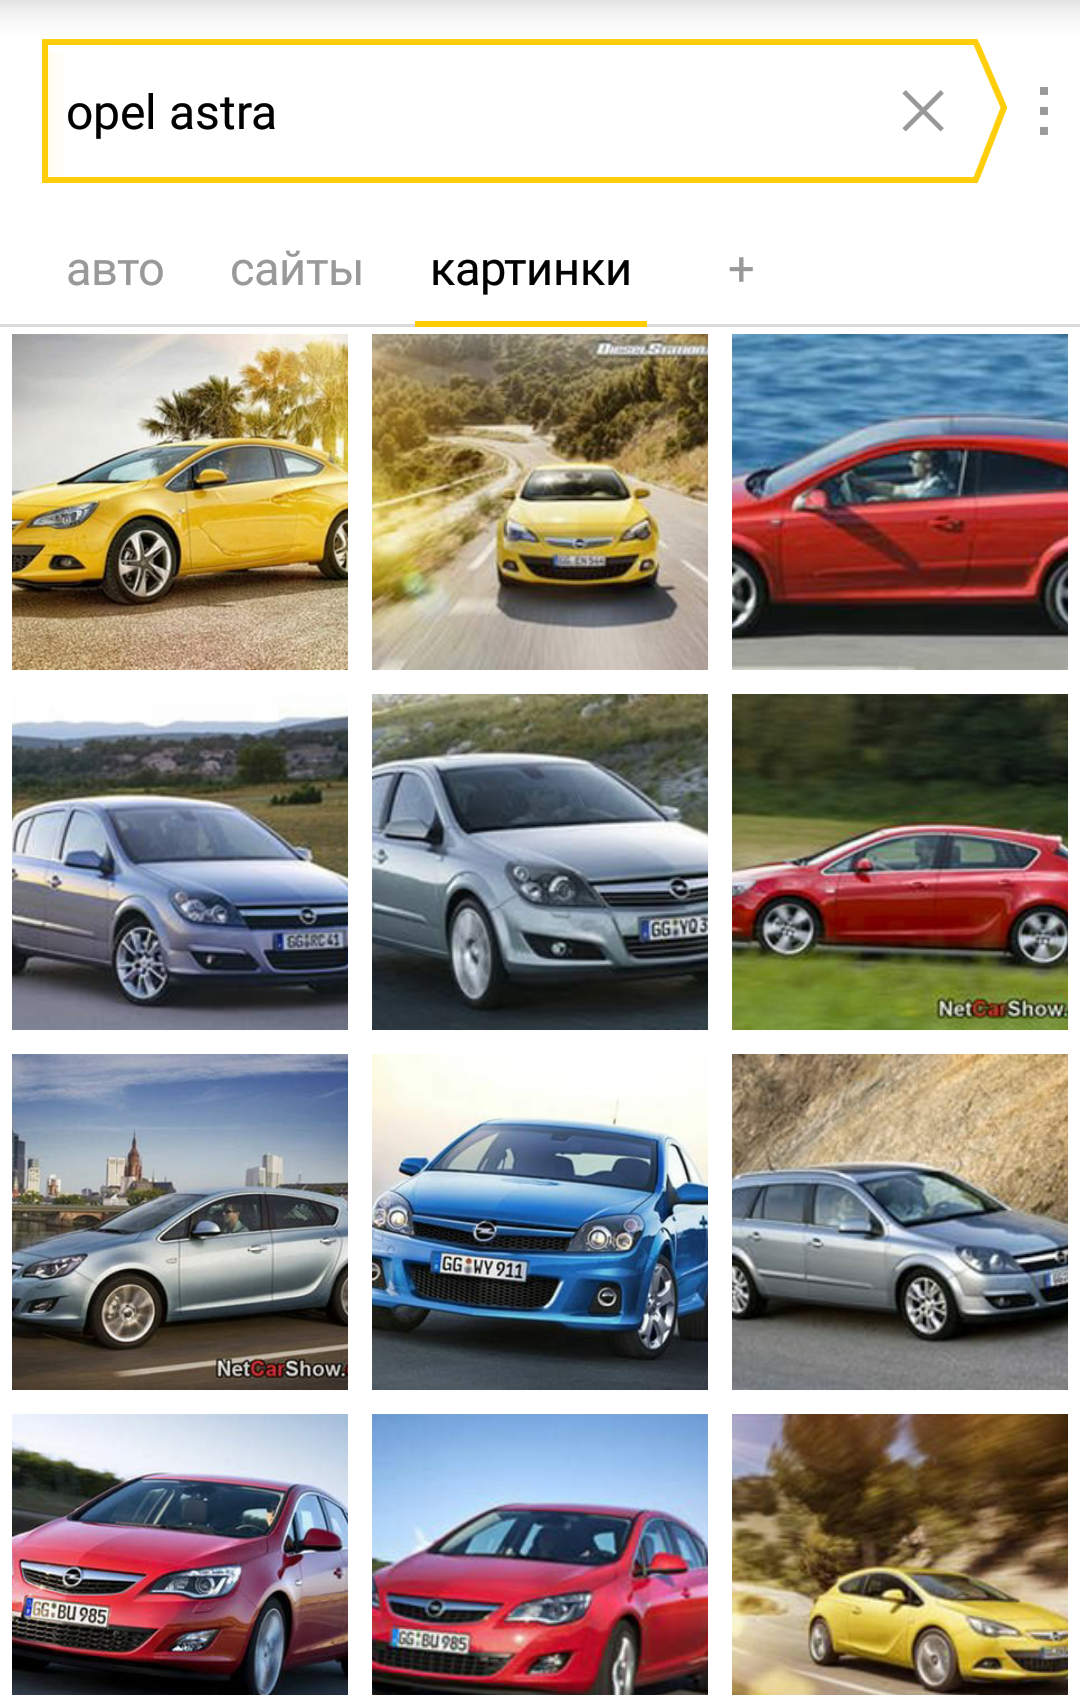
\includegraphics[width=0.3\textwidth]{pics/MultiPageSerp-Yandex-3.png}
  \caption{Выдача мобильного приложения поисковой системы Яндекс с результатами поиска на отдельных страницах.}
  \label{yandex-mobile-app-serp}
\end{figure}

В данной работе рассматривается задача ранжирования разнородных результатов поиска и предлагается универсальный метод ее решения. Этот метод может быть применен для ранжирования результатов произвольного вида и для разных моделей поисковой выдачи. Также он не требует экспертных оценок, поскольку основывается на поведении пользователей.   \todonote{Описать, что в каком разделе}. 

%=================================================================
\chapter{Обзор литературы}

Задача ранжирования занимает важное место в информационном поиске, и на эту тему имеется достаточно большое количество публикаций. Однако подавляющее большинство из них относится к задаче ранжирования однотипных объектов (классической задаче ранжирования) \cite{Liu-LR}. При встраивании же специализированных ответов в результаты поиска требуется ранжировать разнородные объекты. Это не дает возможности применить имеющиеся методы решения классической задачи -- главным образом потому, что разнородные объекты нельзя описать одним набором признаков. В связи с этим рассматриваемая задача требует отдельных исследований, которых на данный момент пока не так много.

В этой главе сначала даются краткие сведения о классической задаче ранжирования и основных методах решения. Затем проводится обзор имеющихся на данный момент публикаций, посвященных ранжированию разнородных результатов.

\section{Классическая задача ранжирования}
\subsection{Формулировка задачи}

\todonote{}

\subsection{Обзор методов решения}

\todonote{}

\section{Ранжирование специализированных ответов}

\todonote{}

\subsection{Формулировка задачи}

\subsection{Обзор методов решения}

Наиболее ранние исследования в области смешивания разнородных результатов поиска касаются встраивания одного конкретного специализированного ответа на первое место в поисковой выдаче \cite{Diaz-News, Konig, Li} и встраивания одного из нескольких специализированных ответов так же на первое место \cite{Arguello-VerticalSelection2009, Arguello-VerticalSelection2010, DiazArguello-VerticalSelection}. Однако подобные методы подходят лишь в тех случаях, когда для заданного запроса уместен только один специализированный результат, и этот результат наиболее подходящий из всех остальных. В более поздних исследованиях рассматривается возможность встраивания специализированных ответов на различные позиции в поисковой выдаче \cite{Lefortier-YandexVideo, Ponnuswami, Arguello-CIKM11, Jie-YahooFederationSystem}. 
%В работе \cite{Lefortier-YandexVideo} исследуется встранивание 
Однако методы, предлагаемые в работах \cite{Lefortier-YandexVideo, Ponnuswami, Arguello-CIKM11} не достаточно универсальны -- они предназначены для встраивания какого-то конкретного специализированного ответа, или существенно зависят от специфики используемых специализированных ответов.
Также методы \cite{Ponnuswami, Arguello-CIKM11} используют экспертные оценки. Это делает их применение дорогостоящим и затрудняет регулярное обновление используемых машинно-обученных моделей, необходимое для учета изменений в потоке поисковых запросов.


%=================================================================
\chapter{Описание метода}

\section{Основные идеи}
\section{Статистический критерий полезности поисковой выдачи}
\section{Формальная постановка задачи}
\section{Модель оценки полезности поисковой выдачи}
\section{Алгоритм ранжирования}
\subsection{Базовый алгоритм}
\subsection{``Жадный'' вариант алгоритма}

%\section{Уменьшение числа вариантов расположения результатов}

%=================================================================
\chapter{Программная реализация}

\section{Схема системы ранжирования}
\section{Уменьшение числа обращений к поисковым источникам}
\section{Используемые технологии}

%=================================================================
\chapter{Оценка качества работы метода}

\section{Методы оценки качества поиска}
\subsection{Методы, основанные на экспертных оценках}
\subsection{Методы, основанные на поведении пользователей}

\section{Выбор данных}
\section{Описание результатов}

%=================================================================
\chapter{Вопросы охраны труда}

\section{Общая характеристика санитарно-гигиенических условий труда}
\section{Эргономические требования}
\section{Микроклиматические условия}
\section{Уровень шума}
\section{Системы освещения}
\section{Излучения}
\section{Электробезопасность}
\section{Инженерно-технические мероприятия по созданию благоприятных условий труда}
\section{Методика и приборы контроля параметров среды}

%=================================================================
\chapter*{Заключение}
\addcontentsline{toc}{chapter}{Заключение}

В данной работе предложен новый метод ранжирования разнородных результатов поиска. Его отличительные особенности состоят в следующем:
\begin{itemize}
  \item ранжируемые результаты рассматриваются в совокупности, а не по отдельности;
  \item результаты располагаются в соответствии с критерием полезности, основанным на действиях пользователей на поисковой выдаче. % на странице с результатами поиска?
\end{itemize}
Благодаря этим особенностям метод обладает рядом преимуществ. Во-первых, он универсален: он может быть применен для ранжирования результатов произвольного вида и для разных моделей поисковой выдачи. Во-вторых, он позволяет естественным образом учитывать взаимосвязи между результатами. И в-третьих, он не требует экспертных оценок для обучения. 

% Какие еще преимущества?
% - легкое добавление нового типа результата / результатов от нового источника ?
% Про события, которые считаем успешными?

Предложенный метод был реализован и применен для встраивания 32-х видов специализированных результатов в поисковую выдачу системы Яндекс для мобильных устройств. Встраивались результаты поиска по изображениям, видео, мобильным приложениям, товарам, новостям, результаты гео-поиска и других сервисов компании Яндекс. 

Было оценено качество работы метода по поисковым метрикам, основанным на экспертных оценках и на поведении пользователей. В сравнении с текущим используемым методом было получено улучшение точности показа специализированных результатов на 21.22\% при снижении полноты на 29.21\% и прирост качества по метрике \textit{pfound} на 0.27\%. \todonote{уточнить результаты} \todonote{+ online-метрики}

В процессе реализации метода также была решена задача нахождения заданного числа кандидатов в аргументы максимизации значения функции, представляющей собой ансамбль ``забывчивых'' деревьев решений (oblivious decision trees), по частично вычисленному вектору признаков. Решение этой задачи позволяет избежать обращения к тем поисковым источникам, результаты которых заведомо нерелевантны заданному поисковому запросу. Разработанное решение имеет самостоятельную ценность и может быть применено и в других задачах.

\renewcommand{\bibname}{Список литературы}
\addcontentsline{toc}{chapter}{Список литературы}
\begin{thebibliography}{@}
  \bibitem{Arguello-VerticalSelection2009} J. Arguello, F. Diaz, J. Callan, and J.-F. Crespo. Sources of evidence for vertical selection. // SIGIR 2009, pp. 315–322. ACM, 2009.
  \bibitem{Arguello-VerticalSelection2010} J. Arguello, F. Diaz, and J.-F. Paiement. Vertical selection in the presence of unlabeled verticals. // SIGIR 2010, pp. 691–698. ACM, 2010.
  \bibitem{Arguello-CIKM11} J. Arguello, F. Diaz, and J. Callan. Learning to aggregate vertical results into web search results. // CIKM 2011, pp. 201–210. ACM, 2011.
%  \bibitem{Arguello-Evaluation} J. Arguello, F. Diaz, J. Callan, and B. Carterette. A methodology for evaluating aggregated search results. // ECIR 2011, pp 141–152. Springer Berlin / Heidelberg, 2011.
  \bibitem{Diaz-News}  F. Diaz. Integration of news content into web results. // WSDM 2009, pp. 182–191. ACM, 2009.
  \bibitem{DiazArguello-VerticalSelection} F. Diaz and J. Arguello. Adaptation of offline vertical selection predictions in the presence of user feedback. // SIGIR 2009, pp. 323–330. ACM, 2009.
  \bibitem{Fox-LDTClick} S. Fox, K. Karnawat, M. Mydland, S. Dumais, T. White. Evaluating Implicit Measures to Improve Web Search. // ACM TOIS, 23(2), pp. 147-168, 2005.    
  \bibitem{ESL} T. Hastie, R. Tibshirani, J. Friedman. The Elements of Statistical Learning, 2nd edition. // Springer, 2009.  
  \bibitem{Jie-YahooFederationSystem} L. Jie, S. Lamkhede, R.t Sapra, E. Hsu, H. Song, Y. Chang. A Unified Search Federation System Based on Online User Feedback. // Proceedings of KDD 2013. ACM, 2013.    
  \bibitem{Joachims} T. Joachims. Optimizing Search Engines using Clickthrough Data. // Proceedings of KDD 2002. ACM, 2002.
  \bibitem{Kim} Y. Kim, A. Hassan, R. White, I. Zitouni. Modeling Dwell Time to Predict Click-level Satisfaction. // Proceedings of WSDM 2014.
  \bibitem{ODT} R. Kohavi. Ch. Li. Oblivious Decision Trees, Graphs, and Top-Down Pruning. // IJCAI, pp. 1071-1079, 1995.
  \bibitem{Konig} A. C. K\"{o}nig, M. Gamon, and Q. Wu. Click-through prediction for news queries. // SIGIR 2009, pp. 347–354. ACM, 2009.
  \bibitem{Lefortier-YandexVideo} D. Lefortier, P. Serdyukov, F. Romanenko, M. de Rijke. Blending Vertical and Web results: A Case Study using Video Intent. // ECIR 2014, pp. 184-196.
  \bibitem{Li} X. Li, Y.-Y. Wang, and A. Acero. Learning query intent from regularized click graphs. // SIGIR 2008, pp. 339–346. ACM, 2008.
  \bibitem{Liu-LR} T. Liu. Learning to rank for information retrieval. // Foundations and Trends in Informaton Retrieval, vol. 3, no. 3, pp. 225–331, 2009. 
  \bibitem{Ponnuswami} A. K. Ponnuswami, K. Pattabiraman, Q. Wu,
R. Gilad-Bachrach, and T. Kanungo. On composition of a federated web search result page: Using online users to provide pairwise preference for heterogeneous verticals. //  WSDM 2011, pp. 715–724. ACM, 2011.
  \bibitem{Metrics} M. Sokolova, G. Lapalme. A systematic analysis of performance measures for classification tasks. // Information Processing and Management 45, p. 427–437. Elsevier, 2009.
  \bibitem{White} R. White, J. Huang. Assessing the Scenic Route: Measuring the Value of Search Trails in Web Logs. // Proceedings of SIGIR 2010. ACM 2010.    
\bibitem{Ashmanov} И. Ашманов, А. Иванов. Оптимизация и продвижение сайтов в поисковых системах, 3-е издание. // Спб.: Питер, 2011.
  \bibitem{PFound} А. Гулин, П. Карпович, Д. Расковалов,
И. Сегалович. Оптимизация алгоритмов ранжирования методами машинного обучения. // РОМИП 2009.
  \bibitem{BoostingOverview} А. Фонарев, А. Дьяконов. Обзор алгоритмов бустинга. // МГУ, 2012.
  \bibitem{MatrixNet} Алгоритм машинного обучения MatrixNet. // URL: \url{https://company.yandex.ru/technologies/matrixnet/}. Дата обращения: 3.06.2015.               
\bibitem{IDC-Analytics} International Data Corporation (IDC). The Digital Universe of Opportunities: Rich Data and the Increasing Value of the Internet of Things. // EMC website,
  URL: \url{http://www.emc.com/leadership/digital-universe/2014iview/executive-summary.htm} (дата обращения: 7.05.2015).
\bibitem{SearchHistory} A Brief History of Search Engines. // Webreference website, 
  URL: \url{http://www.webreference.com/authoring/search_history} (дата обращения: 19.05.2015).

\end{thebibliography}

\chapter*{Словарь терминов}
%\addcontentsline{toc}{chapter}{Словарь терминов}

Поисковая система?

Поисковый запрос

Поисковая выдача
%Совокупность результатов поиска, выдаваемых поисковой системой в ответ на запрос, представленная определенным образом называется \emph{поисковой выдачей}.
% Совокупность результатов поиска, выдаваемых поисковой системой в ответ на запрос, представленная определенным образом, называется ... образует \emph{поисковую выдачу}.


Поисковый источник

Специализированный ответ (специализированный результат)

Ранжирование

Тип информации

\end{document}


